\chapter{Linux Network Stack}

\section{Overview}

\begin{wrapfigure}[20]{r}{.35\textwidth}
	\centering
	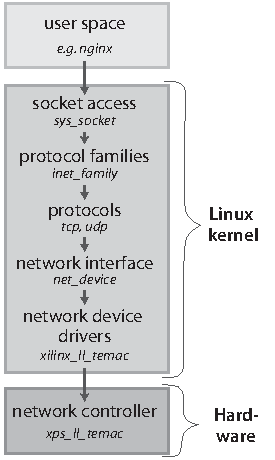
\includegraphics[scale=1]{images/net-stack.pdf}
	\caption{Linux network stack.}
	\label{fig:net-stack}
\end{wrapfigure}
The top most layer of the Linux network stack is the \textbf{system call interface} to create and operate on sockets \cite{netstackana}. The usage of this interface by \textit{nginx} was already described in section \ref{sec:nginx-os-if}. Its purpose is to multiplex networking calls by the user into the kernel \cite{netstackana}. Once a file descriptor was created using the socket interface, data can be exchanged with the network system though general operations on file descriptors like \textit{write} and \textit{read}, too. The socket interface is completely agnostic to different protocols or implementations by network devices and drivers. Its main underlying structure is \texttt{struct sock}, containing all relevant information about a specific socket, like available functions and protocol specific state information.\footnote{\url{http://www.ecsl.cs.sunysb.edu/elibrary/linux/network/LinuxKernel.pdf}} Thereby also protocol and implementation specific functionality is bind to a socket using function pointers (as defined in \texttt{struct inet\_protosw}) \cite{netstackana}.

Whereas the more general data structure \texttt{struct sock} contains mainly meta information about a socket, the major structure for storing data is \texttt{struct sk\_buff}. \textbf{\texttt{sk\_buff}} contains packet data and state information. It is used for to be sent, as well as for received packets almost through out all layers of the network stack. \cite{netstackana}

The gap between protocol handling and device drivers is bridged by the \textbf{network interface} (\textit{netif}) layer. This is a hardware device "agnostic interface layer" \cite{netstackana} with the major purpose of connecting protocols to hardware devices. Information about devices is provided through the \texttt{struct net\_device}. On system start-up all available devices provide register them selves with a filled out \texttt{net\_device} structure. From there on they are know to the network interface layer.

The lowest layer of the network stack being part of the Linux kernel is build by \textbf{device drivers}. These hook into the network interface layer and manage physical/hardware network controllers. For the implemented System on Chip this is the \texttt{xps\_ll\_temac} \gls{ip} core.

Since introduction of the "New API" (NAPI) for communication between device drivers processing packets and the network interface layer, most of the workload for received and to be sent packets is scheduled through software interrupt requests (also known as \textit{soft irq} or \textit{sirq}).\footnote{\url{http://www.linuxfoundation.org/collaborate/workgroups/networking/napi} (as of 12/2012)} During performance tests described in the previous chapter this was visible through high CPU utilization of the \textit{sirq} category.

The network interface layer enqueues \texttt{sk\_buff} packets for transmission using the function \texttt{hard\_start\_xmit(..)}. The device driver pushes received packets to the upper layer using \texttt{netif\_receive\_skb(..)}. \cite{netstackana}